%% =========================================================================
%% Course Report Template (XeLaTex)
%% 
%% Author: 赵苡积 (Yunnan University, School of Information)
%% GitHub: https://github.com/yijizhao
%% 
%% =========================================================================
\documentclass{style/course-report}

\usepackage{subfigure}
\hypersetup{
    colorlinks=true,
    linkcolor=blue,
    filecolor=black,
    urlcolor=black,
    citecolor=blue,
}


% ================= 填写封面信息 =================
\coursetitle{《深度学习》综合实训报告} %课程报告标题
\expname{xxxxx} %题目
\studentname{张三} %姓名
\studentid{20230212} %学号
\major{计算机科学与技术} %专业
\expdate{\today} %日期，默认当天，也可以根据自己需求修改

\begin{document}

% 生成封面
\makecover


\section{选题背景与意义}

描述选题的背景与意义

\section{研究现状}

综述与选题相关的研究现状、存在的问题，除必要的经典开篇之作外，其余文献应尽量以近3年的为主，参考文献样例\cite{Bengio2013,Candes2011,Locatello2019,JTBH202106001,Chen2025IoVCrowdsensing,Higgins2017,Kolda2009,Vapnik1998,Zhang2025Auction}。

\section{问题形式化}

\section{方案设计}
% 本部分需包含关键核心代码（非整个工程代码）、在训练模型时进行的一些关键步骤、参数设置等内容。为了代码片段尽量的美观、统一，建议附代码片段时只附加关键的片段。

\subsection{方案概述}
搭配模型图/总体框架图，描述设计思路、流程等。


\subsection{xxx模块}
分模块介绍：描述、形式化、示意图、核心代码（含关键注释）。

代码样例：

\begin{lstlisting}[language=Python]
# ================= 冒泡排序算法实现 =================
def bubble_sort(arr):
    n = len(arr)
    # 遍历所有数组元素
    for i in range(n):
        # Last i elements are already in place
        for j in range(0, n-i-1):
            # 如果当前元素大于下一个元素，则交换它们
            if arr[j] > arr[j+1]:
                arr[j], arr[j+1] = arr[j+1], arr[j]
    return arr

# 测试代码
if __name__ == "__main__":
    my_list = [64, 34, 25, 12, 22, 11, 90]
    sorted_list = bubble_sort(my_list)
    print("排序后的数组:", sorted_list)
\end{lstlisting}

\subsection{xxx模块}
分模块介绍：描述、形式化、示意图、核心代码（含关键注释）。

\subsection{xxx模块}
分模块介绍：描述、形式化、示意图、核心代码（含关键注释）。


\subsection{算法复杂度分析}
可选，搭配算法伪码描述，进行相应的复杂度分析


\section{实验设置}

\subsection{数据集}
% 如果有数据集（公开数据集/合成数据），需要介绍数据集的相关信息，包括但不限于：数据的来源（有文献源应引用）、数据的基本统计信息、部分数据的可视化、数据的清洗操作、数据标准化、数据增强手段等。

本次实训基于MNIST手写体数据集\cite{lecun2002gradient}，其包含60,000个用于训练的图像样本和10,000个用于测试的图像样本，每张图像为固定大小（28$\times$28像素），像素值为0或1。


\subsection{实验环境}
% 介绍软硬件环境信息等，包括但不限于服务器环境、CUDA版本、语言等信息。


\subsection{模型配置细节}
% 介绍模型超参数的设置范围以及如何选定的超参数，如模型的隐维度、层数、优化器、学习率、总训练轮数、早停轮数、正则系数、dropout率等超参数说明，具体说明如层数$l\in\{1,2,\dots,5\}$，通过网格搜索，并在验证集上设置早停确定最佳超参为xxx。

\subsection{基准方法}
% 你主要模型要对比的方法对象（如果有就保留，没有就删除）

\subsection{评价指标}
% 简介用什么样的指标来评判你的实验结果，比如准确率等指标的简介、定义（含形式化）

\begin{equation}
    \mathrm{ACC} = \frac{A}{B}
    \label{eq:acc}
\end{equation}


\section{实验结果与分析}
% 实验结果包括程序运行结果以及对结果的分析，合理利用折线图、柱状图、表格等多样化的手段丰富实验结果，并且结合结果进行适当的分析。

\subsection{性能比较}

示例表格样式如下：
\begin{table}[H]
    \centering
    \caption{实验结果数据表} % 每个表格应有编号和标题，编号和标题应写在表格上方正中
    \begin{tabular}{ccc}
        \toprule
        参数 & 准确率 / \% & 训练时间 / s \\ % 表格中量与单位之间用“/”分隔
        \midrule
        设置 A & 92.5 & 120 \\
        设置 B & 95.1 & 180 \\
        \bottomrule
    \end{tabular}
    \label{tab:example}
\end{table} % 表格应为三线表

推荐使用python中的matplotlib绘图，加入自动裁剪命令，存为pdf，dpi设为300，注意图中文字应尽量使用中文。单图示例样式如下：
\begin{figure}[H]
    \centering
    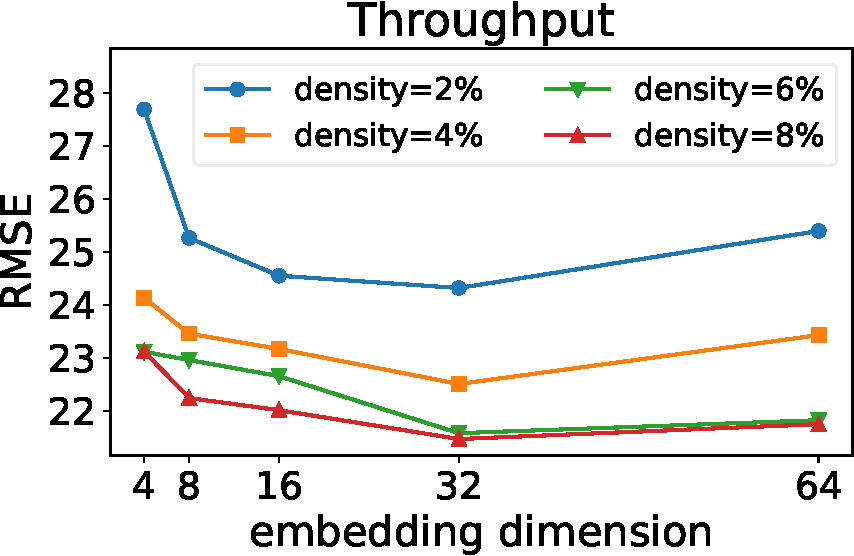
\includegraphics[width=0.70\textwidth]{figs/example.pdf}
    \caption{xxx曲线}
    \label{fig:example}
\end{figure}

多图并列示例图表样式如下：
%%%%%%%%%%%%%%%%%%%%%%%%%%%%%%%%%%%%%%%%%%%%
%                 Figure                  %
%%%%%%%%%%%%%%%%%%%%%%%%%%%%%%%%%%%%%%%%%%%%
\begin{figure}[ht]
    \centering
    \subfigure[XXX1曲线]{
        \label{fig:example_a}
        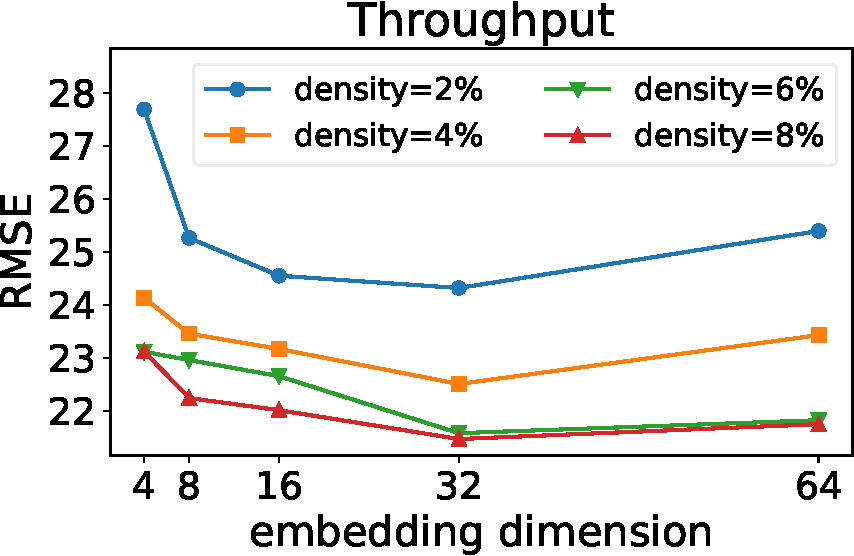
\includegraphics[width=0.45\linewidth]{figs/example.pdf}
    }\hfill
    \subfigure[XXX2曲线]{
        \label{fig:example_b}
        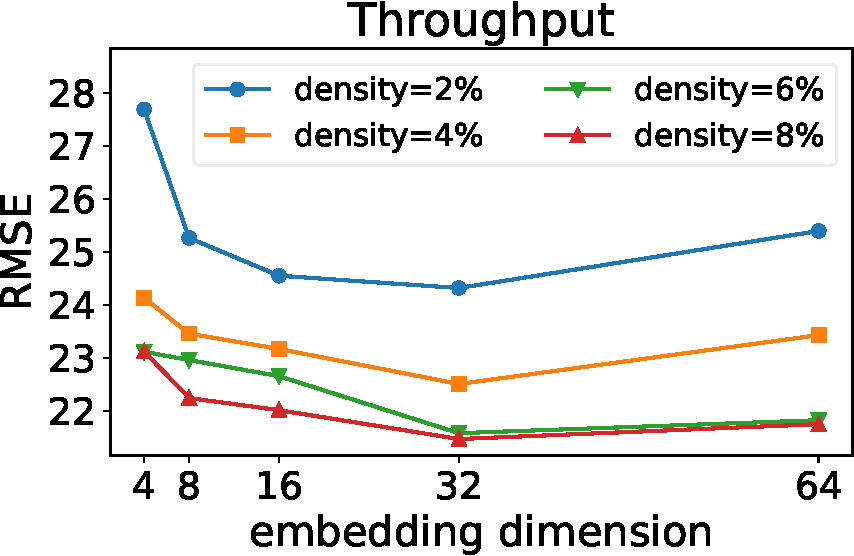
\includegraphics[width=0.45\linewidth]{figs/example.pdf}
    }\hfill
    \subfigure[XXX3曲线]{
        \label{fig:example_c}
        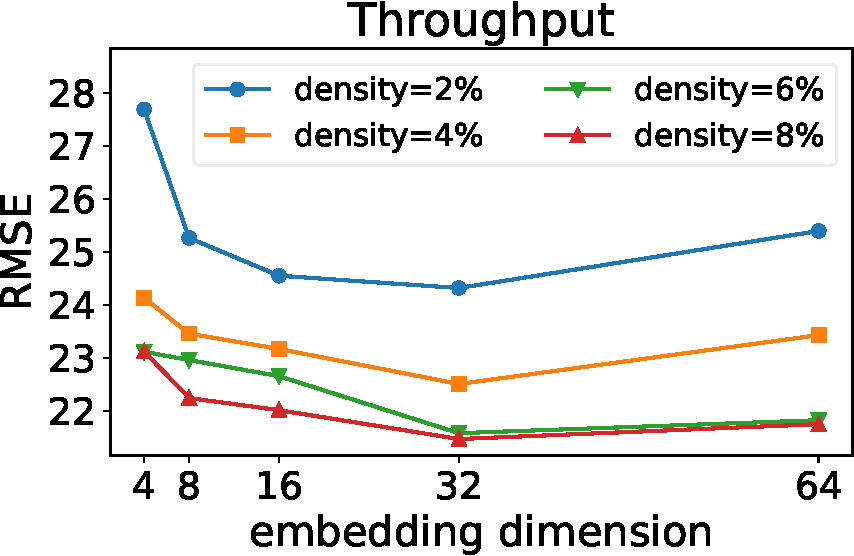
\includegraphics[width=0.45\linewidth]{figs/example.pdf}
    }\hfill
    \subfigure[XXX4曲线]{
        \label{fig:example_d}
        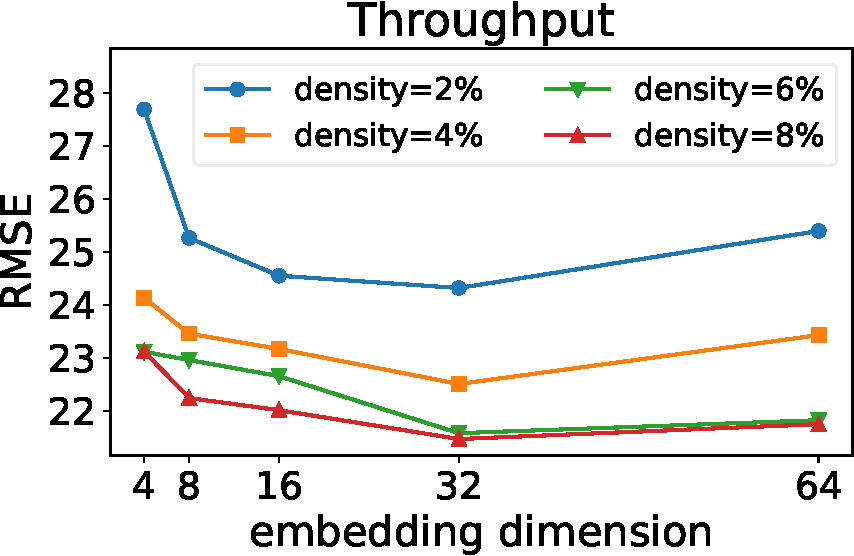
\includegraphics[width=0.45\linewidth]{figs/example.pdf}
    }
    \caption {\label{fig:multi1}嵌入维度的影响.}
\end{figure}

图、表、公式、算式等，一律用阿拉伯数字分别依序连续编排序号，其标注形式应便于互相区别，可分别为：图\ref{fig:example}、图\ref{fig:example_a}、表\ref{tab:example}、公式\ref{eq:acc}等。

\subsection{超参数影响分析}

\subsection{消融实验}

\subsection{效率分析}

\subsection{可视化分析}

\section{心得体会}
% 本部分主要包含自己做实验过程中遇到的困难以及解决办法，通过做实验自己有哪些收获和体会，以及不足等等。


 
\bibliography{ref}
% 参考文献主要包含实验过程中涉及到的参考资料或者借鉴别人的材料等，如无可删除本节。 



\end{document}